\documentclass[11pt]{amsbook}
\setlength{\textwidth}{160mm}
\setlength{\textheight}{220mm}
\setlength{\oddsidemargin}{0mm}
\setlength{\evensidemargin}{10mm}
\setlength{\topmargin}{-10mm}
\newcommand{\REF}{\nopagebreak\noindent{\large{\bf
      References}}\vspace{.2in}}

\newcommand{\Ref}[1]{\medskip\noindent\hangafter=1
      \hangindent=20pt\ignorespaces #1}
\def\X{\scriptscriptstyle X}
\def\Z{\scriptscriptstyle Z}
\usepackage{graphics}
\usepackage{latexsym}
\begin{document}


\noindent
University of Illinois \hfill Department of Economics \\
Fall 2008 \hfill {\large  Economics 508} \hfill Roger Koenker

\vspace{4mm}
\begin{center}

\large{
{\bf Lecture 2\\
Transformations and the Specification of Econometric Models
}}
\end{center}

\vspace{10mm}
A fundamental aspect of interpreting any parametric statistical model is
choice of functional form.  Let's begin a consideration of this topic with 
the following simple example.  Suppose
$$
\log y_i = \alpha + \beta \log x_i + u_i
$$
but unaware of this convenient formulation we instead estimate
$$
y_i = a + bx_i + v_i.
$$
What relationship does $(\hat a , \hat b)$ bear to $(\alpha, \beta)$ in the 
original model and can we hope to say anything reasonable having made this 
initial specification error?

In Figure 1, we can examine a specific version of this situation in 
which $(\alpha, \beta) = (1, .5)$ and the variance of $u_i$ is quite small.
Clearly we don't do a very good job of estimating the curve 
represented by the observed points by the line indicating the least 
\renewcommand{\thefootnote}{\fnsymbol{footnote}}
%%%When you want to go back to the numbers
%%%%\setcounter{footnote}{0}
%%%%then start with footnote 1.
squares fit, but it is useful to look at this more carefully.\footnote{One way 
to do this is to ask:  suppose the $x_i$'s are generated randomly from
some distribution, $F$, and that $E(y|x) = g(x)$, then ($\hat a, \hat b)$ 
solves $\min E_x(g(x) - a - bx)^2$, i.e., $\hat a + \hat b x$ is the best 
linear approximation to $g(x)$ in quadratic mean.}    On a more 
optimistic note it might appear that the slope of the linear fit
might provide a decent approximation to the tangent of the curve 
at a point roughly corresponding to $\bar x.$
\begin{figure}[hbt]
\begin{center}
\resizebox{.8\textwidth}{!}{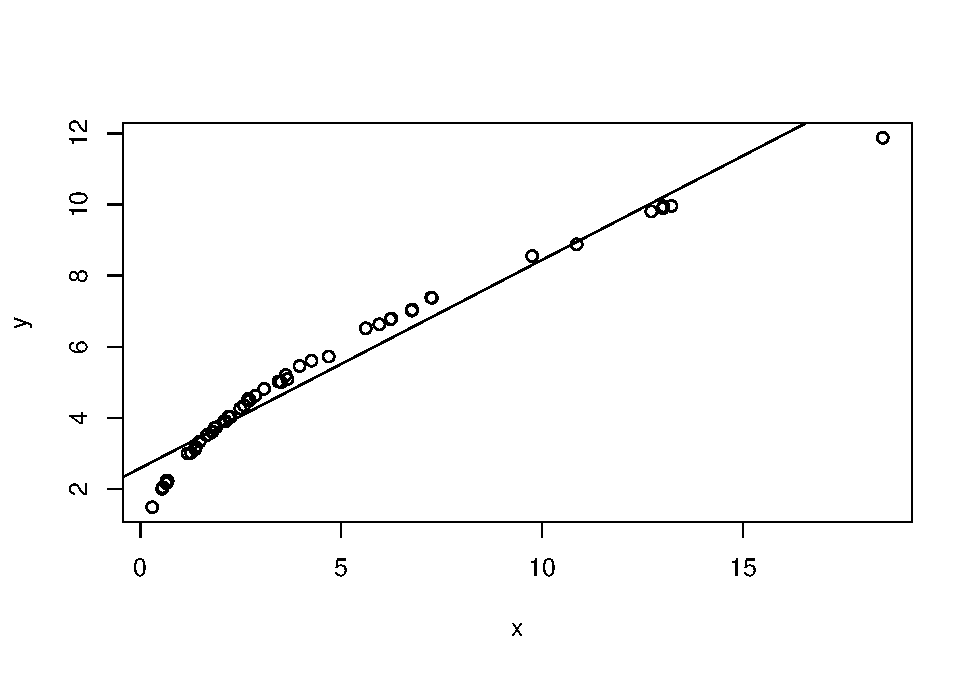
\includegraphics{loglin1.pdf}}
\end{center}
\caption{A linear fit to a log-linear model:  The figure illustrates 50
observations from a log-linear model and a superimposed least-squares
linear fit of the observations.  Note that the fit provides a rough
estimate of the tangent of the curve near the ``center'' of the $x$'s,
but cannot be considered very reliable unless the range of the $x$'s
is quite restricted.}
\end{figure}
\begin{figure}[hbt]
\begin{center}
\resizebox{.8\textwidth}{!}{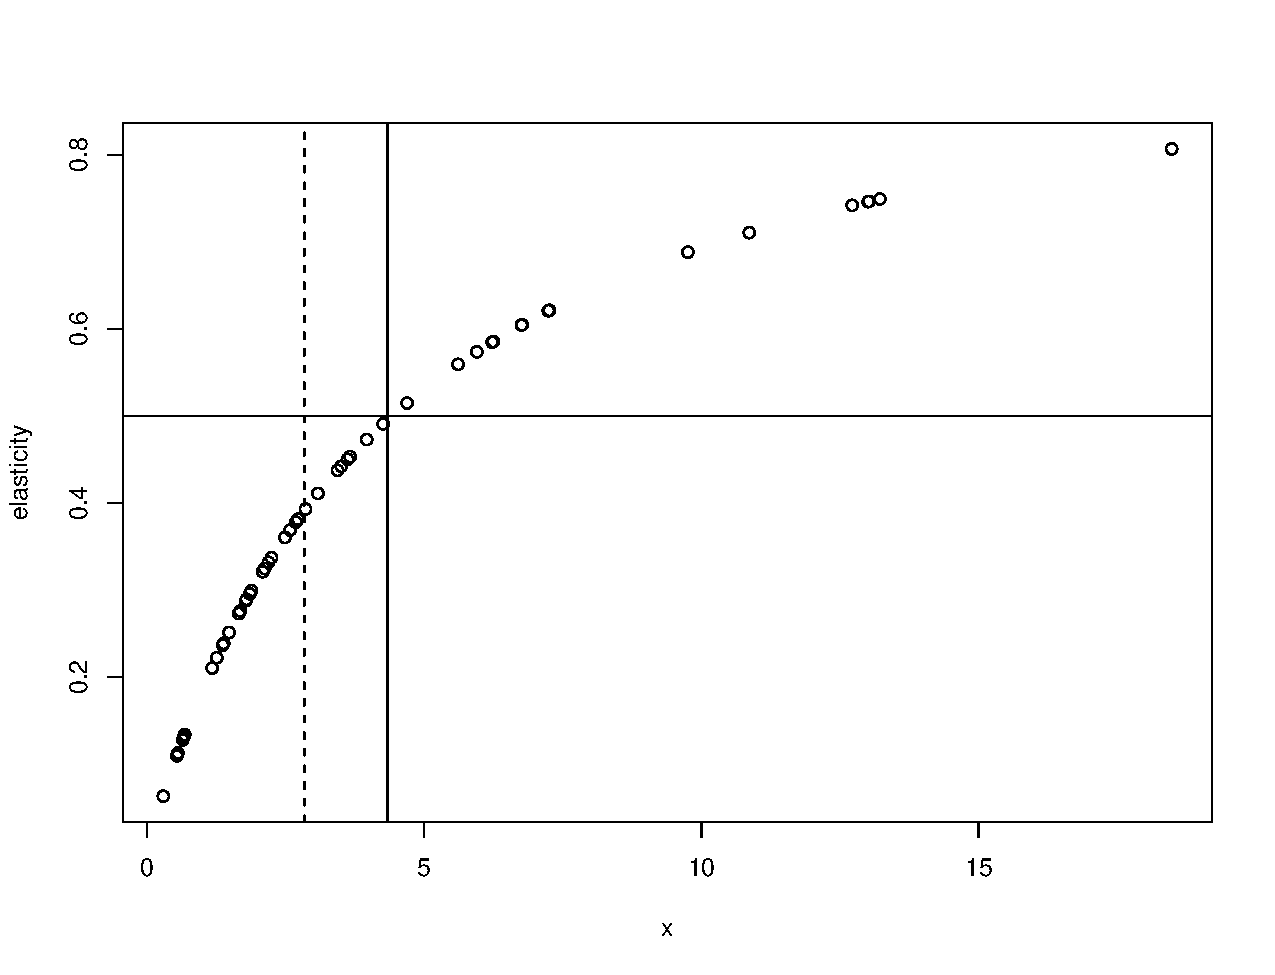
\includegraphics{loglin2.pdf}}
\end{center}
\caption{A linear fit to a log-linear model:  This figure illustrates 
the bias introduced in estimating the elasticity parameter of the log-linear
model by using the estimated linear model.  The points in the figure represent
elasticities implied by the fitted {\it linear} model
at each of the observed $x$'s.  The horizontal line at 
$\beta = .5$ represents the true, constant elasticity for the model,
and the two vertical lines indicate the mean (solid) and geometric mean
(dotted) of the $x$'s.
Thus,  at the mean of the $x$'s the linear model slightly overestimates
the elasticity, and at the geometric mean it slightly underestimates it.}
\end{figure}
Figure 2 illustrates this phenomenon on the elasticity scale.  
Were we to estimate the log-linear model we would have an easily 
interpreted constant elasticity estimate.  However, since we have estimated 
the model in the linear form, the implied elasticity of $y$ with respect to $x$
varies as we move along the fitted line.  More explicitly, the elasticity is 
defined as
$$
\eta = \frac{dy}{dx} \enskip \frac{x}{y}
$$
and according to the linear specification the derivative, $dy/dx = b$ 
is constant, so the natural estimate of the elasticity of $y$ with 
respect to $x$, at any point $x$, is given by
$$
\hat\eta(x) = \hat b \cdot \frac{x}{\hat y(x)}
$$
where $\hat y(x) = \hat a + \hat b x.$  If we were going to offer 
only one such elasticity estimate for expository purposes, we would typically
choose $x = \bar x$, but sometimes it is useful to choose several such points
of evaluation for purposes of comparison.  Recall $\hat y (\bar x) = \bar y$
as long as the estimated model has an intercept. This is done for each of 
the observed values of $x $ in Figure 2.  The horizontal line at 
$\beta =.5$ is the ``true'' elasticity according to which the data 
was generated, while the dots represent $\hat\eta(x)$ at 
the various deserved $x$'s.  Obviously these estimates are rather poor
in the extremes, but reasonably good in the center of the $x$'s.  
The two vertical lines represent the arithmetic and geometric means of $x$
and we note that one yields a small overestimate while the other
yields a small underestimate of $\beta$.  This is the first of many lessons
which can be roughly formulated by the 

\vspace{5mm}
\noindent {\em Maxim:}  It is dangerous to draw inferences too far away 
from the center of your data.

A corollary, which is often offered as advice to young novelists is 
``Write what you know,'' another pithy corollary is ``Extrapolate at your 
peril.''  A nice introduction to a more general formulation of these
issues is White (1980).

Having seen this example it is natural to ask whether there is a 
systematic strategy for deciding on appropriate functional forms.  This is 
obviously a big topic and I will try only to briefly survey the basic
idea in the simplest bivariate regression setting.

The classical approach to dealing with this `\`transformation problem'' 
involves the family of power transformations
$$
h(x, \lambda) = \left\{ \begin{array}{cl}
\frac{x^\lambda-1}{\lambda} & \lambda \neq 0\\
\log x & \lambda=0
\end{array} \right.
$$
Applying this transformation to the response variable $y$ and/or the
independent variable(s) $x$ yields a rich class of  potential models.
It is useful to consider a few special cases.  We will consider 
$\lambda = 0$ which is somewhat peculiar in detail, but $\lambda = -1$
is also of interest.


\noindent{\em Exercise:}  Verify using L'H\^opital's rule that
$$
\lim_{\lambda\rightarrow 0} \frac{x^\lambda - 1}{\lambda} = \log x
$$

\noindent{\em Answer:}  
\begin{eqnarray*}
\lim_{\lambda \rightarrow 0} \frac{x^\lambda - 1}{\lambda} &=& 
\frac{\frac{d}{d\lambda} (e^{\lambda \log x} - 1)}{1} |_{\lambda= 0} \\
&=& e^{\lambda \log x} \cdot \log x|_{\lambda=0}\\
&=& \log x
\end{eqnarray*}
\begin{figure}[hbt]
\resizebox{.8\textwidth}{!}{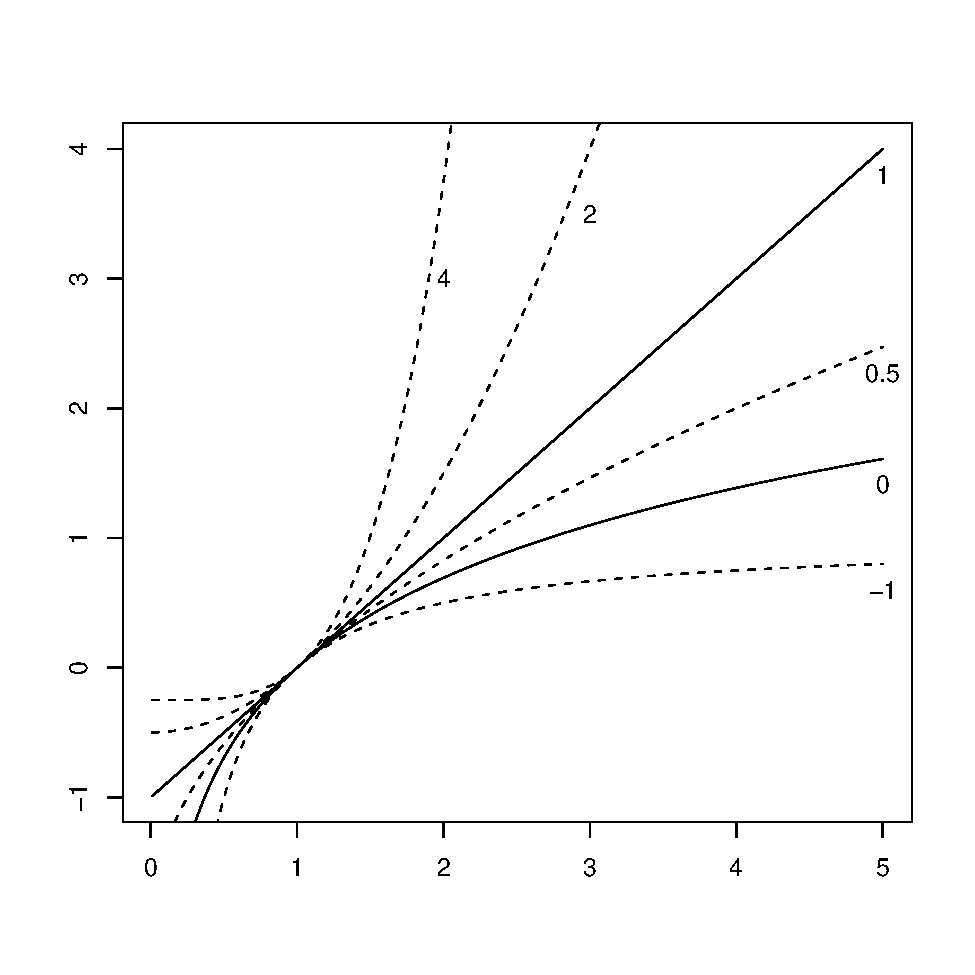
\includegraphics{links.pdf}}
\caption {The Box-Cox Power Transformations:
The Figure illustrates 6 versions of the Box-Cox Power family of
transformations.  Note that the log transformation fits nicely
into the family with $\lambda =0$.  
}
\end{figure}
\begin{figure}[hbt]
\resizebox{.8\textwidth}{!}{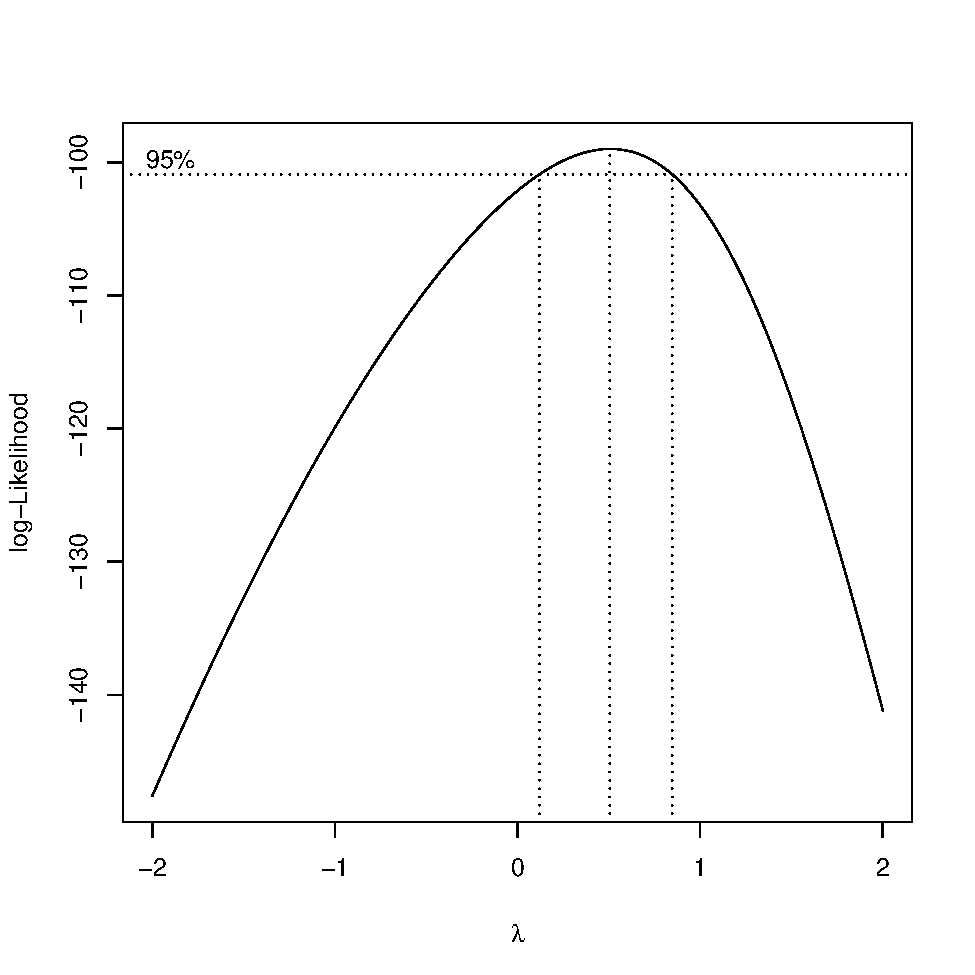
\includegraphics{like2.pdf}}
\caption {The Box-Cox Power Transformation:
The Figure illustrates the profile log likelihood for a simple
bivariate linear model, the confidence interval indicated for
$\lambda$  is based on the asymptotic theory of the likelihood
ratio statistic.
}
\end{figure}
The family of Box-Cox transformations is illustrated in Figure 3 for 6 
different values of $\lambda.$  
The family is quite flexible and useful, but it is somewhat limited
because it is only fully applicable for $x \geq 0.$  It has been 
suggested that one might extend the definition using
$$
\lambda(x) = (|x|^\lambda \mbox{ sgn }(x) -1)/\lambda
$$
but this behaves rather strangely and is rarely used in applications.

As an exercise in reviewing some basic ideas about maximum likelihood 
estimation, let's consider,  following Box and Cox (1964), the problem of 
estimating the model
$$
h(y_i, \lambda)  = x_i\beta + u_i
$$
assuming that $\{u_i\}$ is iid ${\mathcal N} (0, \sigma^2)$.  
The log likelihood is
$$
\ell (\beta, \lambda, \sigma) = - \frac{n}{2} \log (2\pi \sigma^2) - \frac{1}{2\sigma^2} \sum(h( Y_i , \lambda ) - x_i\beta)^2 + \log |J|
$$
where $J = \prod_{i=1}^n |\partial h (y_i)/\partial y_i|$ is the 
determinant of the transformation from $u$ to $h(y, \lambda).$  Note that
$$
\frac{\partial h(y_i, \lambda)}{\partial y_i} =  y_i^{\lambda-1}
$$
so 
$$
\log |J| = (\lambda -1) \sum_{i=1}^n \log (y_i). 
$$

Concentrating the likelihood we have 
$$
\ell (\lambda, \sigma) = -\frac{n}{2} \log \hat\sigma^2 + \log |J| + K
$$
where $K$ doesn't depend on the parameters.  Now note that if we had been
very lucky and  the response observations $y_i:  i = 1, ... , n$ happened
to have geometric mean of zero, then the Jacobian term would have been
zero.  Alternatively, suppose we, with malice aforethought, transform the
observed $y_i$'s:  $y_i \rightarrow \tilde y_i \equiv y_i / \tilde y$
where $\tilde y = (\prod y_i)^{1/n} $ denotes the geometric mean of $y_i$'s.
Then,
\[
\log |J| = (\lambda -1) \sum \log (\tilde y_i ) = 
(\lambda -1) \sum \log (y_i / \tilde y ) = 
(\lambda -1) \sum (\log (y_i) - log( \tilde y )) = 0.
\]
How convenient!  Having made this transformation the Jacobian term vanishes
and we can focus on the simple classical idea of  minimizing the sum of
squared errors, or equivalently, minimizing $\log (\hat \sigma^2)$ since
it becomes the only  relevant term in the likelihood.  One might still worry
about whether there are any serious side effects resulting from the transformation
of the response observations?  A useful exercise would be to convince yourself
that a.)  in the case that $\lambda = 0$ so we had the $\log$ transformation
then dividing by the geometric mean would have only the effect of shifting the intercept
of the model, or b.) in the case that $\lambda = 1$, dividing the $y_i$'s by
a constant rescales {\it all} the coordinates of the  $\hat \beta$ vector 
by the same factor.  These so-called ``equivariance'' properties of the 
least-squares estimator will arise periodically throughout the course.

The function $\ell(\lambda)$ which we used to call the concentrated log 
likelihood we now call the profile (log) likelihood, terminology I believe 
introduced by Cox.  The profile likelihood provides an extremely convenient 
and powerful means of doing inference in many problems.  In the simple Box-Cox
problem under consideration we would often like to test the hypothesis 
$H_0: \lambda = \lambda_0$. This is effectively done using the fact (whose
proof is deferred to 476) that under $H_0$,
$$
\tau (\lambda_0 ) = 2(\ell(\hat \lambda) - \ell(\lambda_0) ) \leadsto \chi_1^2 \leqno (*)
$$
where $\hat\lambda$ denotes the maximum likelihood estimate of $\lambda.$
The limiting behavior of this likelihood ratio statistic can also be used
to construct confidence intervals for $\lambda$:  we simply find the set 
of $\lambda_0$ such that $\tau (\lambda_0) $ fails to reject at a 
specified level of confidence.  This is illustrate in Figure 4.

%\input fig3-4.tex

Sometimes we would rather not go to the bother of estimating the Box-Cox
model, but instead we would like to estimate some ``preferred'' form and
then test whether this choice of $\lambda$ is reasonable. 
A simple test suggested by David Andrews (1971) handles this situation, 
and since it nicely illustrates an important principle of diagnostic test
design we will develop it in some detail.  Consider
$$
h(y, \lambda) = x_i^\top \beta + u_i
$$
with $\lambda =1$ as our ``preferred'' value.  Expanding in Taylor series 
we have 
\begin{eqnarray*}
h(y, \lambda) &\simeq& y-1 + (\lambda - 1) \frac{d h(y,\lambda)}{d\lambda}
|_{\lambda=1} \\
&=&  (y-1) (\lambda-1) [ y \log y - (y-1) ]
\end{eqnarray*}
Thus, for $\lambda$ close to one,
$$
y-1 \simeq x^\top \beta + (\lambda -1) y \log y
$$
this seems rather strange since it suggests that we should regress
$y$ on $y \log y $ -- this is clearly unsound.  But if we instead proceed 
in two steps:
\begin{enumerate}
\item Estimate the linear model and compute $\hat y_i = x_i\hat \beta $ 
for $i=1, \ldots, n$ and then
\item Reestimate the augmented model
$$
y_i = x_i^\top \beta + \gamma \hat y_i \log \hat y_i
$$
and test $H_0: \gamma = 0$.
\end{enumerate}
This procedure, in effect provides one-step approximation to the mle for $\lambda$
i.e., $\hat\lambda = \hat\gamma +1.$

\vspace{5mm}
\noindent{\em Question:}  What about the 1? Is it really needed, if so how
would it affect the result if you ignored it?

\vspace{5mm}
\noindent{\em Exercises} (Review)  For the OLSE $\hat\beta$ show
(1.) $\hat\beta (\sigma y + X\gamma, X) = \sigma\hat\beta (y, X) + \gamma$, 
and 
(2.) $\hat \beta (y, XA) = A^{-1} \hat\beta(y, X).$

On the other hand if $H_0: \lambda =0$ is the preferred version, then at
$\lambda = 0$, we have,
$$
\frac{dh(y,\lambda)}{d\lambda}|_{\lambda=0} = \frac{1}{2}(\log y)^2
$$
so now we would fit
$$
\log(y) = x^\top \beta+\delta \cdot (\widehat{\log y})^2
$$
so here $\delta $ estimates $(1/2) \lambda$ under the alternative hypothesis.

Another useful and important aspect of diagnostic evaluation of transformation
models is the partial residual plot.  We illustrate this for the gasoline
data of PS 2 in the next two figures.  In the first group of 4 figures
I plot in the upper two figures the scatterplots of percapita US gasoline
demand vs percapita income and price respectively.  Note that neither of
these plots look like something a reasonable person would want to fit
with a straight line.  Nevertheless, we need to become accustomed to
the idea that the {\it multivariate} relationship may be approximately
linear even if the bivariate relationships are not.  In this case this
is (encouragingly!) roughly true.  

\begin{figure}[hbt]
\begin{center}
\resizebox{.8\textwidth}{!}{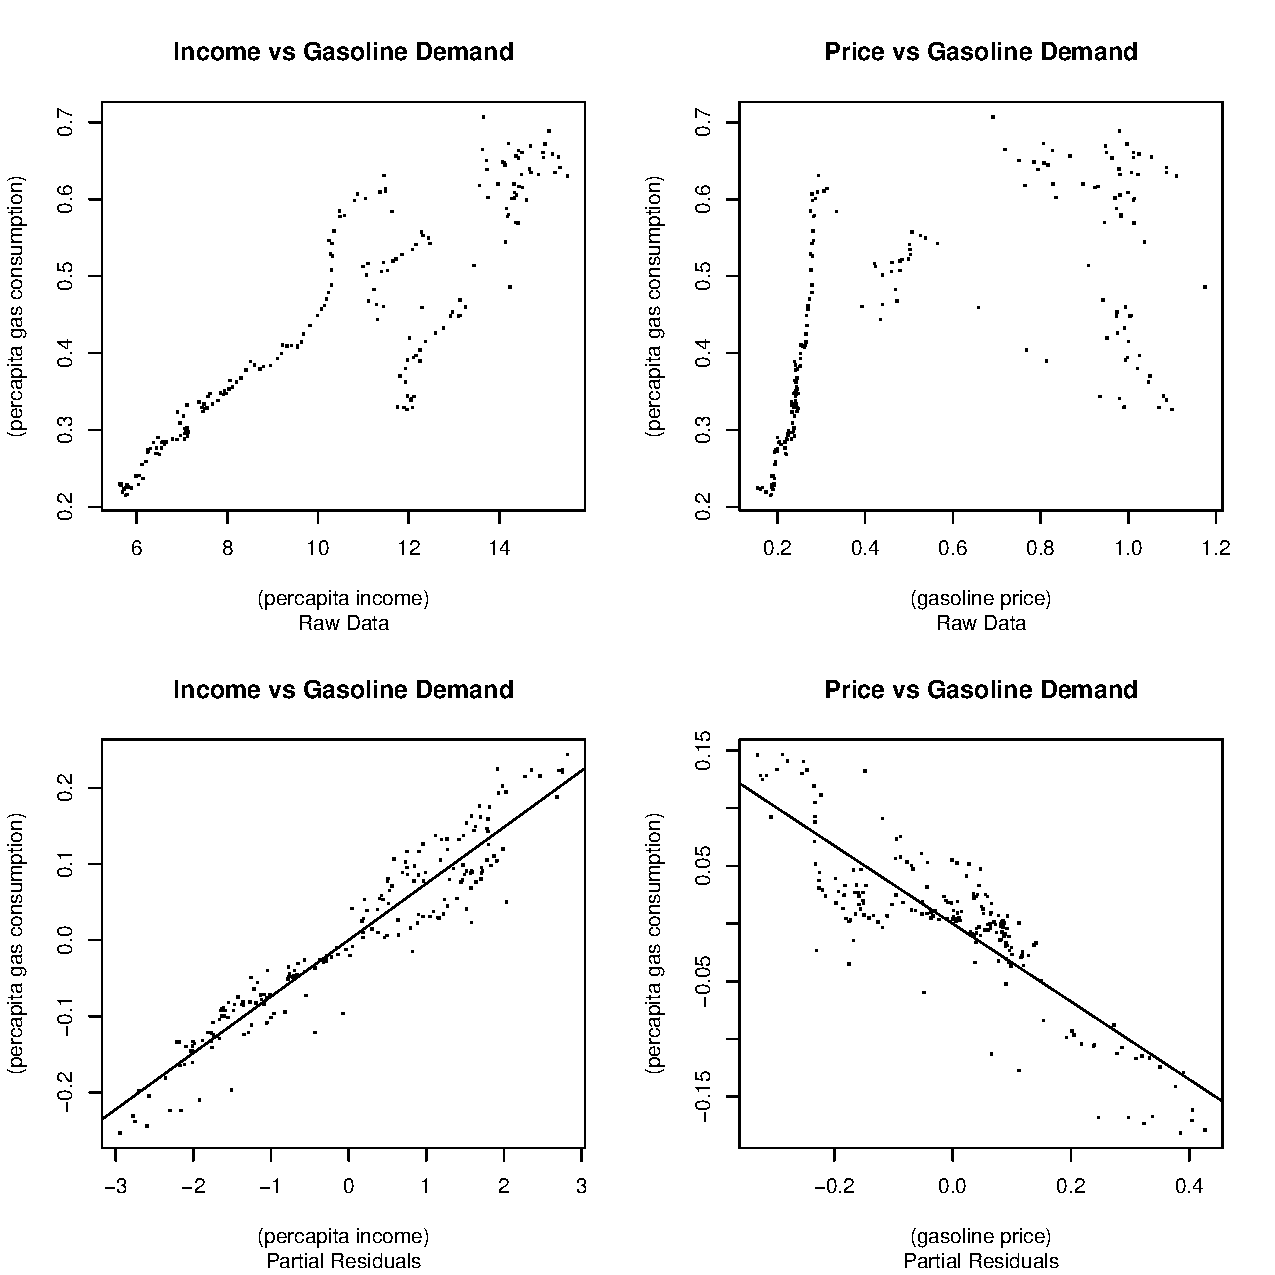
\includegraphics{prraw.pdf}}
\end{center}
\end{figure}

\begin{figure}[hbt]
\begin{center}
\resizebox{.8\textwidth}{!}{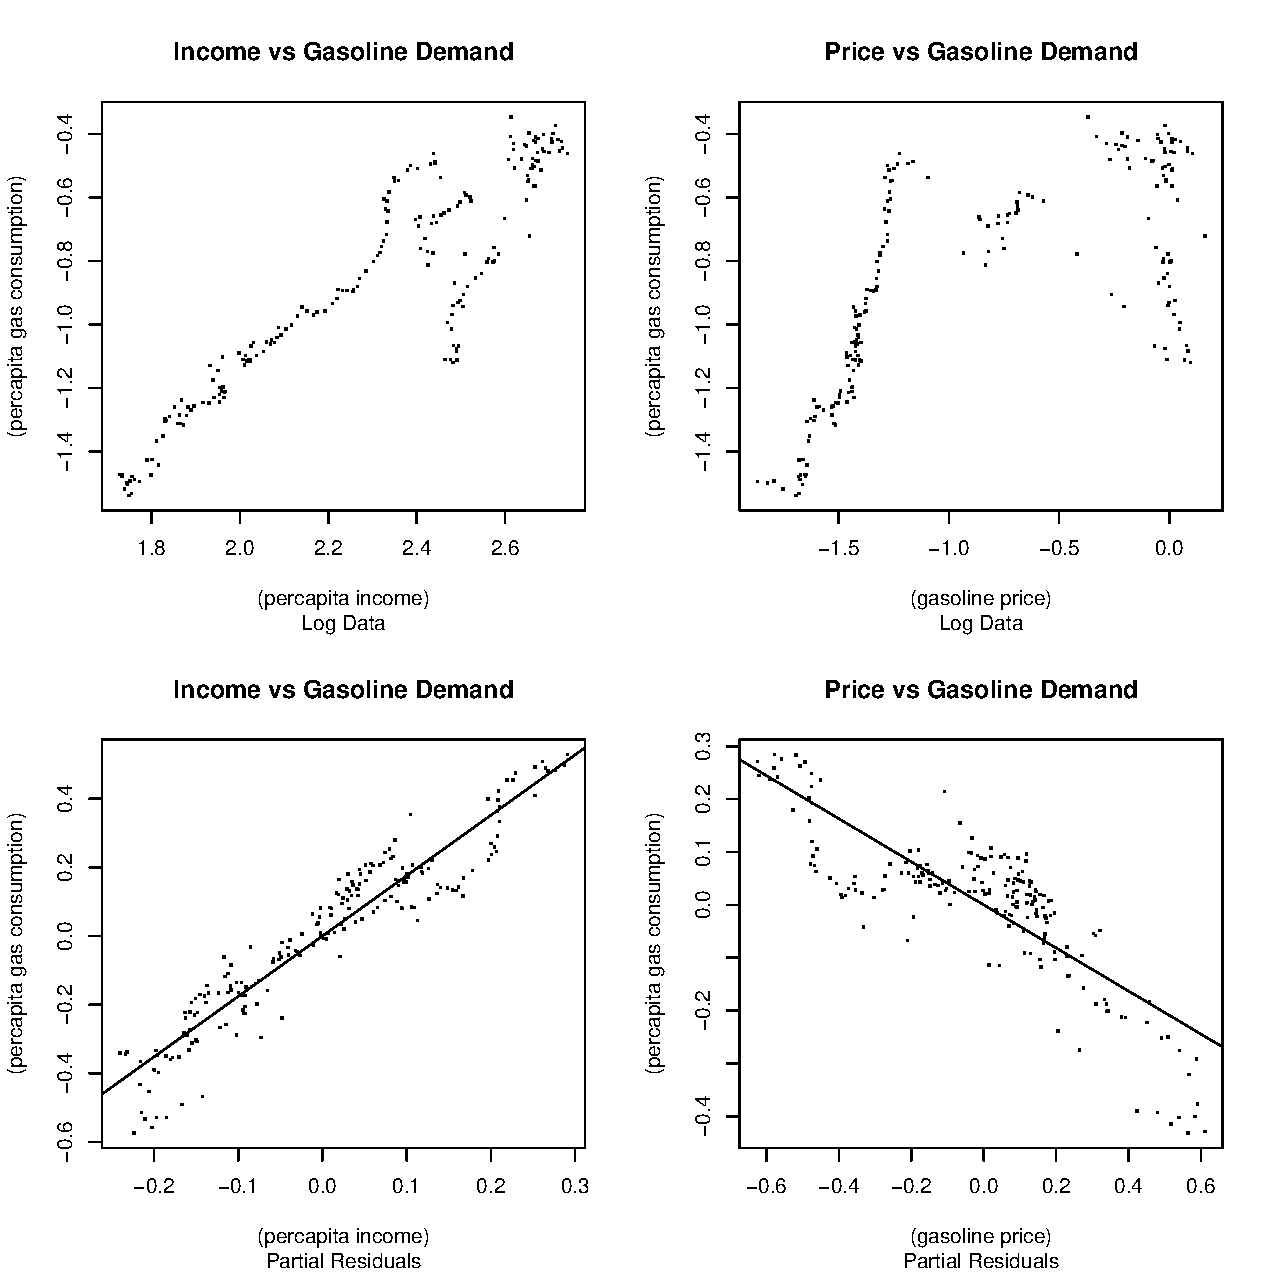
\includegraphics{prlog.pdf}}
\end{center}
\end{figure}

The partial residual plot is a device for representing 
the final step of a multivariate regression result
as a bivariate scatterplot.  To accomplish this slightly mysterious feat,
we need somehow to ``remove'' the effect of the ``other''
variables before doing the scatterplot.  The natural way of doing this
is to regress the two variables of primary interest 
on the ``other'' variables of the model, and then plotting the
resulting residuals against one another.  This can be formalized in
the following way.

Consider the model
$$
y=X\beta + z\gamma + u
$$
and the least squares fitted values,
$$
\hat y = X \hat \beta + z \hat \gamma
$$
where $M_{\X} = I-P_{\X}, $ and $P_{\X} = X(X^\top X)^{-1}X^\top$ 


\noindent{\em Theorem}  (Gauss-Frisch-Waugh)  
$\hat\gamma=(z^\top M_{\X} z)^{-1}z^\top  M_{\X} y$
where $M_{\X} = I-P_{\X}, $ and $P_{\X} = X(X^\top X)^{-1}X^\top X.$

\noindent{\em Proof} Write
$$
z^\top M_{\X} \hat y = z^\top M_{\X}X\hat\beta + z^\top M_{\X} z\hat\gamma
$$
but $M_{\X} X = 0$, so it only remains to show that 
$$
z^\top M_{\X} P_{\Z} y = z^\top  M_{\X} y
$$
where $Z = [X\vdots z]$.  Note that
$$
M_{\X} P_{\Z} = (I-P_{\X}) P_{\Z} = P_{\Z} - P_{\X}P_{\Z} = P_{\Z} - P_{\X}.
$$
In the last step note that $X^\top P_{\Z} =(P_{\Z}X)^\top  = X^\top$  (Why?) so 
$P_{\X}P_{\Z} = P_{\X}.$  Finally, we can compute,
$$
z^\top M_{\X} P_zy = z^\top (P_{\Z} - P_{\X})y = z^\top y - z^\top P_{\X} y  = 
z^\top (I-P_{\X})y = z^\top M_{\X} y
$$
which concludes the argument.

An additional feature of this approach is that the standard errors that
would be computed by the last step are exactly the same as those that
come out the of full regression.  So not only does the scatter plot
give an accurate assessment of the position of the least squares fit
of the bivariate relationship, it also provides an accurate visual
assessment of the precision of this estimate.

This last point inevitably recalls an amusing  
``fiasco of econometrics'' perpetrated  here
by Robert Barro in his 1997 David Kinley lecture.  
Barro presented some ``growth regressions'' of the type described in
his monograph with Sala i Martin.  But to illustrate the results for
a ``general audience'' he chose to spend a considerable portion of the
talk showing slides of the bivariate relationship between various
explanatory variables and his ``national growth'' variable, after
controlling for the effect of other variables.  Barro's approach
was, however, somewhat idiosyncratic.  For each of the possible $z$ variables
of interest, he computed $\tilde y = \hat u + z_i \beta_i$, that is
the residuals from the full regression plus the estimated effect
of the $i$th variable, and then this variable was centered at zero
and plotted against $z_i$.  This approach is easily shown to produce
the correct point estimate of the coefficient $\hat \beta_i$, 
(it would be a useful exercise for students to show this),
however the visual impression of the scatterplot is much more optimistic
than one would expect to get from the partial residual plot method
described above.  In effect, the denominator effect in the t-statistics
of $z_i^\top  M_X z_i$
is replaced in the Barro approach by $z_i^\top  M_1 z_i$ -- regression on only an
intercept.  Since the former can be very small, compared to the later
the result is a picture that has an implied standard error that appears
considerably smaller than would the standard error in the full regression.
In the next panel of two figures, I illustrate the effect of the Barro
approach for the gasoline data.  As one can see, these figures suggest
a much more precise estimate of the two effects than that conveyed by
the conventional partial residual plots appearing above. 
This is good, of course, if the object is to impress the audience with
the precision of the fit, but bad if one is interested in conveying
an accurate assessment of that precision.

\begin{figure}[hbt]
\begin{center}
\resizebox{.8\textwidth}{!}{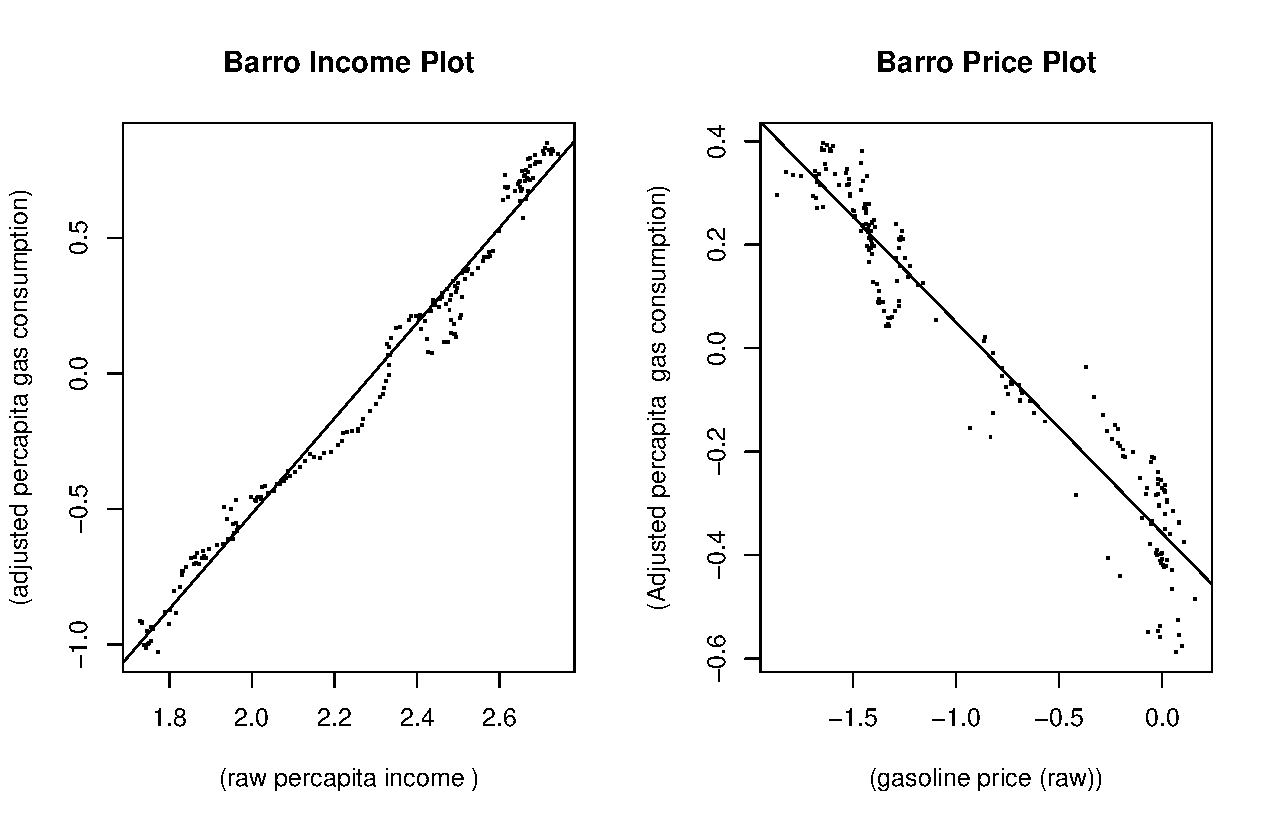
\includegraphics{barro.pdf}}
\end{center}
\end{figure}

 

\vspace{.5in}
\begin{center}
{\em Conflicting Objectives of Transformations}
\end{center}

We have 3 possibly conflicting objectives in choosing a transformation.  
We would like the transformation to (simultaneously) yield a model
\begin{tabbing}
yield a model which is \= (iii)(1) \= homoscedastic \kill
\> (i) \> which is linear in parameters\\
\>(ii)\> homoscedastic\\
\>(iii)\> has approximately ``normal'' conditional density
\end{tabbing}
Carroll and Ruppert have proposed a more general strategy which they call 
``transforming both sides''.  We begin with a model like
$$
E(y_t | x_t)  = f(x_t, \beta).
$$
One might think of this as the {\em systematic} part of the model before 
any noise is introduced.  Now we might consider models based on the Box
Cox transformation of the form,
$$
h(y_t, \lambda) = h(f(x_t, \beta), \lambda) + u_t
$$
But this is different than the Box-Cox models we considered above.
Here $f(x_t, \beta)$ is intended to deal with the non-linearity, 
while $h$ is {\em hopefully} going to transform to homoscedastic and 
normal errors.  How does $h(\cdot)$ work?

Suppose $y_i$ has $E(y_i|x_i) = \mu_i, V(y_i|x_i) = \sigma_i^2$ and
$\sigma_i = \sigma g(\mu_i)$, then
\begin{eqnarray*}
V(h(y_i)) &\simeq& E(h(y_i) - h(\mu_i))^2\\
&\simeq& (h'(\mu_i))^2 E(y_i-\mu_i)^2\\
&=& (h'(\mu_i))^2 \sigma^2(g(\mu_i))^2
\end{eqnarray*}
Note these approximations depend on $\sigma$ being ``small!''
This is our first contact with the so-called $\delta$-method, but
it will appear in various guises throughout the course.
Now, if we were to choose $h$ so that
$$
h'(\mu_i) = \frac{1}{g(\mu_i)}
$$
then we would have (approximate) homoscedasticity.  For example,
in Poisson cases
$$
g(\mu) = \mu^{1/2}
$$
so 
$$
h(\mu) = 2\mu^{1/2} \Rightarrow h'(\mu) = \frac{1}{\mu^{1/2}}
$$
and 
$$
g(\mu) = \mu \Rightarrow h(\mu) = \log (\mu) \Rightarrow h'(\mu) = \frac{1}{\mu}
$$
and
$$
g(\mu) = \mu^{(1-\lambda)} \Rightarrow h(\mu) = y^{(\lambda)} \Rightarrow h'(\mu) = \mu^{\lambda-1}
$$
Here we use the common notational convention that 
$y^{(\lambda)} = (y^\lambda -1)/\lambda$.
Another way to look at this is to say that if $\sigma^2$ is small relative to 
the variability of $\mu_i$'s, then
$$
h(y_i) = h(\mu_i) + h'(\mu_i)(y_i-\mu)
$$
For this order of approximation we are back to a ``simple'' 
heteroscedastic model,
$$
y_i = \mu_i + \sigma h'(\mu_i) \varepsilon_i
$$
Note that the interpretation of the $\beta$'s is quite different in this 
setup than in the classical Box-Cox setup.  There the $\beta$'s
don't mean much independent of $\lambda$ -- recall $\partial y / \partial x$
expression, -- but here they do.


\vspace{5mm}
\noindent Transformation {\em and} weighting:  Consider the model
$$
h(y_i, \lambda) = h(f(y_i, \beta), \lambda) + \sigma g(\mu_i(\beta), 
z_i \theta)\varepsilon_i
$$
Now we can think of $g(\cdot)$ as modeling the heteroscedasticity and 
$h(\cdot)$ being exclusively for achieving normality, while $f(\cdot) $ 
fixes the non-linearity in the conditional mean relationship.
This model is considerably more complicated to estimate, but may arise
naturally in the process of diagnostic checking.

\vspace{5mm}
\begin{center}
{\em Interpreting Transformed Models}
\end{center}

It is very important to be clear about what parameters ``{\em mean}'' in
transformation models, 

In the normal linear model
$$
y_i = x_i  \beta + \sigma \varepsilon_i \qquad \varepsilon_i \sim {\mathcal N}(0, 1)
$$
$$
P(y_i < y|x_i) = \Phi ((y-x_i\beta)/\sigma)
$$
$$
Q_{y_i}(p|x_i) = x_i\beta + \sigma\Phi^{-1}(p)
$$

%\input fig1-2.tex

In the Box-Cox framework we have,
$$
h(y, \lambda) = x_i\beta + \sigma\varepsilon
$$
$$
\mbox{so the $p$th quantile of $y_i|x_i$ is } \qquad \qquad  y_i = h_\lambda^{-1} (x_i\beta + \sigma\varepsilon)  \qquad\qquad \qquad \qquad\qquad \qquad \qquad \qquad 
$$
$$
Q_{y_i} (p|x_i) = h_\lambda^{-1} (x_i\beta + \sigma\Phi^{-1}(p))
$$
Thus if we wanted to estimate the effect of a change in $x_{ij}$ on 
the $p$th quantile of $y_i$, we would write
$$
\frac{\partial}{\partial x_{ij}} Q_{y_i} (p |x_i) = \frac{\partial}{\partial x_{ij}}
[h_\lambda^{-1} (x_i\beta + \sigma\Phi^{-1}(p))]
$$
For example, if 
$$
h_\lambda (y_i) = \frac{y_i^\lambda -1}{\lambda}
$$
then,
\begin{eqnarray*}
y_i^\lambda &=& \lambda h_i+1\\
y_i &=& (\lambda h_i+1)^{1/\lambda}\\
Q_{y_i} (p|x)&=& (\lambda(x_i\beta + \sigma\Phi^{-1} (p) ) +1)^{1/\lambda}\\
\frac{\partial y_i}{\partial x_{ij}} &=& \frac{1}{\lambda} (\lambda(x_i\beta + \sigma\Phi^{-1} (p) ) +1)^{\frac{1}{\lambda} - 1} \cdot \lambda \beta_j = 
(\lambda(x_i\beta + \sigma\Phi^{-1} (p) ) +1)^{\frac{1}{\lambda} - 1} \beta_j
\end{eqnarray*}
This could then be used to generate a confidence interval.
Note that models for expectations are less convenient here since 
$E(h(y)) \neq h(Ey)$.

\vspace{5mm}
\begin{center}
{\em Transformations for Proportions}
\end{center}

Often we are interested in estimating models of proportions, for example, 
Engel Curves for proportions of expenditure,  unemployment rates, etc.
Two simple alternatives are logit: 
$h(y) = \log (y/(1-y))$  or more generally $ h(y, \lambda) = y^\lambda - 
(1-y)^\lambda$  folded power transformation.
Note $\lim_{\lambda\rightarrow 0} h(y, \lambda) = \log (y/(1-y))$
We will have more to say about these cases later in the term.

\vspace{5mm}
\noindent {\em References}

\Ref Andrews, D. A note on the selection of data transformations, 
{\it Biometrika}, 58, 249-54.

\Ref Box, G.E.P. and D.R. Cox (1964),  Analysis of Transformations, (with discussion), {\em JRSS(B)}, 26, 211-52.

\Ref Carroll, R. and D. Ruppert (1988),  {\em Transformation and Weighting in Regression}, Chapman-Hall.

\Ref White, H. (1980), Using least squares to approximate unknown regression 
functions, {\em IER}, 21, 149-170.

\end{document}
